\section{Programación en Python}

El objetivo de este curso es enseñar a utilizar como herramienta el lenguaje de programación Python para usuarios con conocimientos previos de programación.

\subsection{Codificación de las instrucciones}

Para que una computadora lleve a cabo alguna acción, debe leer las instrucciones guardadas en la memoria y ejecutarlas en el CPU, tal como se muestra en la imagen \ref{graf:componentes-computador}\footnote{\cite{Stallings2005} pp. 61}.

\begin{figure}[ht!]
   \centering
   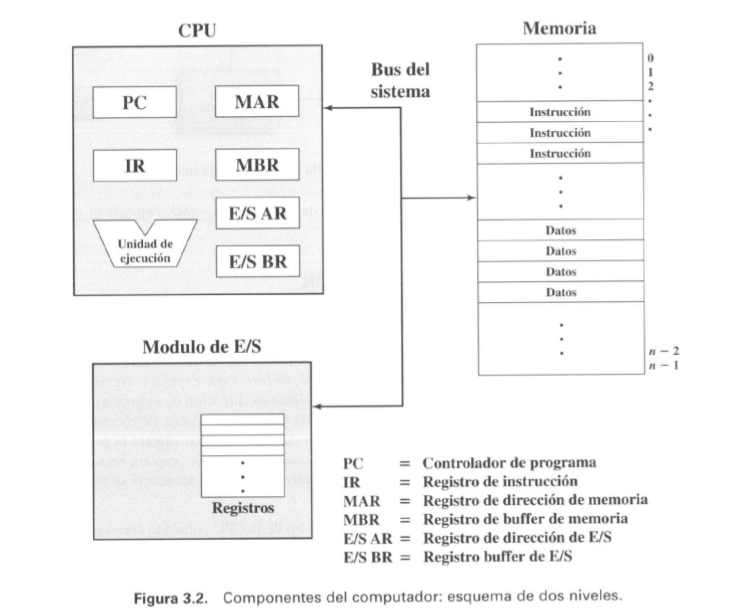
\includegraphics[scale=0.4]{imagenes/estructura_computadora.png}
   \caption{Componentes del computador}\label{graf:componentes-computador}
\end{figure}

Estas instrucciones están codificadas en código binario (ceros y unos), también llamado \textit{lenguaje binario}. No solo las operaciones aritméticas, sino también los símbolos utilizados por las computadoras son representados por el estándar ASCII (American Standard Code for Information Interchange).  La correspondencia entre secuencias de bits y caracteres determinada
por la tabla es arbitraria. La letra ``a", por ejemplo, se codifica con la secuencia de bits 01100001 y la letra ``A" se codifica con 01000001. Todo texto se puede codificar como una secuencia de bits, por ejemplo el texto ``Hola'' es:\\

\begin{center}
01001000 01101111 01101100 01100001
\end{center}

En la pantalla de texto (el famoso ``modo DOS'' o más propiamente dicho ``Interfaz de Linea de Comandos'') se ven los símbolos ASCII originales, pero en las pantallas gráficas, ahora utilizadas de forma masiva, lo que se ven son símbolos gráficos formados por pixeles, donde el color de cada pixel está dado por una combinación de ceros y unos.

\subsection{Programar}

Tal como se mencionaba en la sección anterior, las instrucciones para que una computadora realice alguna acción están almacenadas en memoria. La memoria es una especie de ``almacén'' con cajones numerados donde se almacenan instrucciones para el CPU. Cada ``cajón", está numerado o mejor dicho, tiene su propia dirección de memoria. \\

La CPU lee las direcciones memoria en forma secuencial (a menos que una instrucción le indique lo contrario) y ejecuta lo que cada instrucción le señala. Cada instrucción describe acciones simples como sumar dos direcciones de memoria, copiar una dirección en otra, empezar a leer a partir de una determinada dirección y así por el estilo.\\

Combinando instrucciones se pueden lograr resultados complejos, y esas instrucciones son un programa. La secuencia de instruccciones que la CPU puede ejecutar se llaman \textit{código de máquina}, el cuál codifica instrucciones en secuencia de unos y ceros que hacen al CPU ejecutar determinadas acciones.\\

\subsection{Lenguaje ensamblador}

En el inicio de los tiempos, cuando las computadoras eran gigantes que ocupaban pisos enteros, hechas de cables y tubos de vacio, hacer un programa implicaba volver a cablear, donde cada cable en un panel de conectores significaba un uno y el cable desconectado era un cero. Para evitar esta labor tediosa, se crearon abreviaciones para conjuntos de instrucciones, estos \textit{códigos mnemotécnicos} son abreviaturas fáciles de recordar.\\

Por ejemplo un programa que busque obtener el promedio de tres números, sería como sigue:\\

\begin{pyglist}

SUM #10, #11, #13
SUM #12, #13, #13
DIV #13, 3, #13
FIN
\end{pyglist}

Donde SUM suma los números en las posiciones 10 y 11 y los coloca en la posición 13, luego suma el número en la dirección 12 al número en la dirección 13 y los coloca en la posición 13, luego se divide el número en la dirección 13 entre 3 y se almacena el resultado en la dirección 13, obteniéndose el resultado.\\

Este código es llamado \textit{lenguaje ensamblador}, y el programa que lo traduce a código máquina es el \textit{ensamblador}. Debido a que las instrucciones varían por cada familia de procesadores, el lenguaje ensamblador es diferente y los programas escritos para un tipo de CPU no funcionarán en otro.

\subsection{Lenguajes de programación}

Para evitar este carnaval de lenguajes ensambladores y además simplificar la programación, se crearon los lenguajes de alto nivel, los cuales son iguales en todas las plataformas donde se ejecutan, de ahí su calificativo de ``alto nivel". En contraste el código de máquina y los lenguajes ensambladores son lenguajes de bajo nivel por su dependencia de un hardware específico.\\

Por ejemplo, en Python el programa que divide tres valores es:

\begin{pyglist}
media = (10 + 11 + 12)/3
\end{pyglist}

Mucho más sencillo que sus equivalente en lenguajes de bajo nivel. 

\subsection{Compiladores e interpretes}

Para que los lenguajes de alto nivel tengan independencia de la plataforma, se ejecutan mediante programas llamados compiladores e interpretes, los cuáles se encargan de los detalles del hardware y presentan la misma interfaz a un programa escrito en el mismo lenguaje en otra plataforma.\\

Por ejemplo, se puede escribir un programa Python en una Machintosh y volverlo a ejecutar en una PC con Windows o en un servidor con FreeBSD y obtener el mismo resultado.\\

En palabras de \cite{Marzal2003}: \footnote{\cite{Marzal2003} pp. 14}

\begin{quotation}
\textit{Un \textbf{compilador} lee completamente un programa en un lenguaje de alto nivel y lo traduce en su integridad a un programa de código de máquina equivalente. El programa de código de máquina resultante se puede ejecutar cuantas veces se desee, sin necesidad de volver a traducir el programa original.}\\

\textit{Un \textbf{intérprete} actúa de un modo distinto: lee un programa escrito en un lenguaje de alto nivel instrucción a instrucción y, para cada una de ellas, efectúa una traducción a las instrucciones de código de máquina equivalentes y las ejecuta inmediatamente. No hay un proceso de traducción separado por completo del de ejecución. Cada vez que ejecutamos el programa con un intérprete, se repite el proceso de traducción y ejecución, ya que ambos son simultáneos.}
\end{quotation}

De lo escrito, se puede deducir que un programa compilado es en general más veloz que un programa interpretado, debido a que el intérprete debe ejecutarse siempre que se corre el programa. Por otro lado, los lenguajes interpretados han sido diseñados para ser más flexibles y dinámicos, automatizando la gestión de la memoria y liberando al programador de tareas que dificultan su trabajo.

\subsection{Algoritmos}

Dos programas que resuelvan el mismo problema de la misma forma, así estén escritos utilizando diferentes lenguajes de programación, están siguiendo ambos el mismo algoritmo. Un algoritmo es en esencia, una secuencia de pasos para conseguir un objetivo.\\

Por ejemplo, el algoritmo de la media de tres números es:

\begin{enumerate}
\item Solicitar el valor del primer número,
\item Solicitar el valor del segundo número,
\item Solicitar el valor del tercer número,
\item Sumar los tres números y dividir el resultado por 3,
\item Mostrar el resultado.
\end{enumerate}

Esta secuencia de instrucciones nos permite conseguir el objetivo en cualquier lenguaje de programación, idependientemente de las instrucciones que se necesiten. Son procedimientos que se pueden ejecutar, siguiendo la línea de razonamiento, sin necesidad de tener una computadora, utilizando papel o una calculadora.\\

No todo conjunto de instrucciones es un algoritmo, para tener esa condición un procedimiento debe cumplir las siguientes condiciones: \footnote{\cite{Marzal2003} pp. 21}

\begin{enumerate}
\item Ha de tener cero o más datos de entrada.
\item Debe proporcionar uno o más datos de salida como resultado.
\item Cada paso del algoritmo ha de estar definido con exactitud, sin la menor ambiguedad.
\item Ha de ser finito, es decir, debe finalizar tras la ejecución de un número finito de pasos, cada uno de los cuales ha de ser ejecutable en tiempo finito.
\item Debe ser efectivo, es decir, cada uno de sus pasos ha de poder ejecutarse en tiempo finito con unos recursos determinados (en nuestro caso, con los que proporciona una computadora).
\end{enumerate}

Además de lo anterior, se busca que los algoritmos sean eficientes, es decir, que logren su objetivo lo más rápido posible.

\section{¿Qué es Python?}

Python es un lenguaje de programación de alto nivel, fácil de aprender y de uso profesional con una sintaxis legible y ordenada. Posee además un entorno interactivo que permite hacer pruebas con velocidad y despejar dudas sobre el lenguaje. Su entorno de ejecución detecta muchos errores y proporciona información para resolverlos. En cuanto a sus características como lenguaje, Python puede programarse funcionalmente u orientado a objetos y posee ricas estructuras de datos que facilitan la labor del programador.\\

Python es muy utilizado en ámbitos científicos y de ingeniería debido a las características mencionadas y a la disponibilidad de librerías matemáticas y científicas de gran calidad.\\

Python puede ser ejecutado en múltiples plataformas, incluyendo las más comunes como Windows, Linux y MacOS. Se pueden llevar a cabo programas de escritorio, desarrollo web, utilitarios, juegos, etc.\\

Actualmente Python es utilizado por diversas empresas nacionales y extranjeras para escribir utilitarios, sistemas de información y desarrollos web.\\

Un ejemplo de programa Python es el siguiente:\\

\begin{pyglist}
#!/usr/bin/python
# -*- coding: utf-8 -*-

a = float(raw_input('Dame un numero:'))
b = float(raw_input('Dame otro numero:'))
c = float(raw_input('Y ahora, uno mas:'))
media = (a + b + c) / 3
print 'La media es', media                        
\end{pyglist}

\subsection{Utilización}

Python es un lenguaje de programación interpretado, dinámico y multiparadigma (POO, estructurado). Se caracteriza por tener una baja curva de aprendizaje, ser multiuso y permitir una programación ordenada y elegante.\\

Su visión está expresada en el Zen de Python:

\begin{center}
\begin{quote}
Bello es mejor que feo.\\
Explícito es mejor que implícito.\\
Simple es mejor que complejo.
\end{quote}
\end{center}

Para empezar a experimentar con Python se puede utilizar el intérprete interactivo desde la consola:\\

\begin{figure}[ht!]
   \centering
   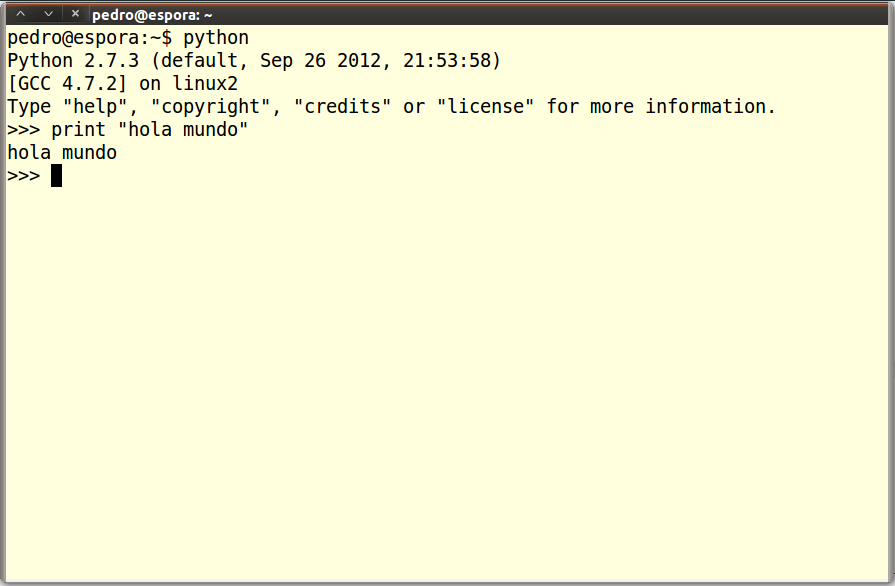
\includegraphics[scale=0.2]{imagenes/consola_python.png}
   \caption{Consola python}\label{graf:consola_python}
\end{figure}


\newpage

Si se desea ejecutar varias lineas de código sin tener que tipear una tras otra en la consola interactiva, se guarda el código en un archivo de texto que termine en .py y se ejecuta utilizando el comando python.

\section{Variables}

Las variables son espacios de memoria a los que asignamos arbitrariamente valores que van a permanecer en la variable mientras no se cierre el programa. Por ejemplo, si deseamos calcular el volumen de un cubo u otro volumen similar, tenemos que multiplicar tres lados del sólido.\\

\begin{pyglist} [language=python]
>>> 123*14.5*12
21402.0
>>> 123*14.5*11
19618.5
>>> 
\end{pyglist}

Solo para cambiar un lado, se tienen que introducir de nuevo todos los números en el problema. Si estos números se hubieran guardado en una variable, volver a llevar cabo el cálculo hubiera sido más sencillo.\\

\begin{pyglist} [language=python]
>>> a = 123
>>> b = 14.5
>>> a*b*10
17835.0
>>> 
\end{pyglist}

Se han creado dos variables, a y b, en las cuales se almacenan dos números que no cambian y solo se debe escribir el nuevo número.\\

Al asignarle valor a una variable, el orden es importante, el valor se asigna de derecha a izquierda.\\

\begin{center}
\textit{variable = expresión}
\end{center}

Se debe recalcar que en un lenguaje de programación como Python, el símbolo $=$ no significa ``igual a'' sino, ``se asigna a''.\\

Para poner nombres a las variables se siguen las siguientes reglas:

\begin{quotation}

El nombre de una variable es su identificador. Hay unas reglas precisas para construir identificadores. Si no se siguen, diremos que el identificador no es válido. Un identificador debe estar formado por letras minúsculas, mayúsculas, dígitos y/o el carácter de subrayado (\_), con una restricción: que el primer carácter no sea un dígito.\\

Hay una norma más: un identificador no puede coincidir con una palabra reservada o palabra clave. Una palabra reservada es una palabra que tiene un significado predefinido y es necesaria para expresar ciertas construcciones del lenguaje.
\end{quotation}

Las palabras reservadas de Python son: \textbf{and, as, assert, break, class, continue, def , del, elif , else, except, exec, finally, for, from, global, if , import, in, is, lambda, not, or, pass, print, raise, return, try, while, with y yield}.


\section{Tipos básicos}

Los tipos básicos son en esencia tres: números, cadenas y valores booleanos.

\begin{itemize}
\item Números: 5 (entero), 4.7 (flotante), 4 + 6j (complejo).
\item Cadenas: ``Clase de programación''.
\item Booleanos: True y False
\end{itemize}

Los comentarios se escriben utilizando el símbolo \#:\\

\begin{pyglist} [language=python]
# Este es un comentario
a = "Esta es una linea de programa"
\end{pyglist}

Las variables se asignan de forma dinámica y dependen del tipo de dato que se les asigna, por ejemplo, una variable puede ser entera, luego asignarsele un valor de coma flotante y por último una cadena y es válido:\\

\begin{pyglist} [language=python]
>>> a = 5
>>> a
5
>>> a = 6.4
>>> a
6.4
>>> a = "Lima"
>>> a
'Lima'
>>> 
\end{pyglist}

\subsection{Cadenas}

Existen tres tipo de cadenas: Las cadenas normales, las cadenas unicode y las cadenas ``crudas'' (raw en inglés).\\

\begin{pyglist} [language=python]
>>> print "a"  
a              
>>> c = r"\n"        
>>> c                          
'\\n'    
>>> print c                     
\n   
>>>      
>>> d = u"g"
>>> d
u'g'
>>> print d
g
>>>     
\end{pyglist}

En Python se pueden concatenar y multiplicar cadenas.\\

\begin{pyglist} [language=python]
>>> 4 * "cad"
'cadcadcadcad'
>>> "cadena1" + " " + "cadena 2"
'cadena1 cadena 2'
>>> 
\end{pyglist}


\subsection{Bool}

Python tiene un tipo de datos especial que permite expresar sólo dos valores: cierto y falso en la forma True o False. Son los valores booleanos, llamados así en honor del matemático inglés George Bool, que desarrolló un sistema algebraico basado en estos dos valores y tres operaciones: la conjunción, la disyunción y la negación. Python ofrece soporte para estas operaciones con los operadores lógicos.\\

Se estudiará con más profundidad este tipo de datos al aprender sobre los operadores lógicos y de comparación en la siguiente clase.

\section{Operadores aritméticos}

\begin{table}[h]
\centering
\begin{tabular}{|c|c|c|} \hline
Operador	             & Descripción & Ejemplo     \\ \hline
+         & Suma               & r = 3 + 2    \# r es 5   \\ \hline
-         & Resta              & r = 4 - 7    \# r es -3   \\ \hline
-         & Negación           & r = -7       \# r es -7   \\ \hline     
*         & Multiplicación     & r = 2 * 6    \# r es 12   \\ \hline
**        & Exponente          & r = 2 ** 6   \# r es 64    \\ \hline
/         & División           & r = 3.5 / 2  \# r es 1.75    \\ \hline
//        & División entera    & r = 3.5 // 2 \# r es 1.0    \\ \hline
\%         & Módulo             & r = 7 \% 2    \# r es 1   \\ \hline
\end{tabular}
\end{table}

Si en una operación utilizamos un número flotante y un entero el resultado será flotante.\\

\section{Ejercicios}

Traducir las siguientes expresiones matemáticas a Python y evaluarlas. Utilizar el menor número de paréntesis posible.

\begin{enumerate}
\item 2 + (3 · (6/2))
\item $\frac{4 + 6}{2 + 3}$
\item $(4/2)^5$
\item $(4/2)^{5+1}$
\item $(−3)^2$
\item $−(3^2)$
\end{enumerate}

Evaluar los polinomios:

\begin{enumerate}
\item $x^4 + x^3 + 2x^2 − x$
\item $x^4 + x^3 + \frac{1}{2}x − x$
\end{enumerate}

Evaluar estas expresiones y sentencias en el orden indicado:

\begin{enumerate}
\item a = 'b'
\item a + 'b'
\item a + 'a'
\item a * 2 + 'b' * 3
\item 2 * (a + 'b')
\item 'a' * 3 + '/*' * 5 + 2 * 'abc' + '+'
\item 2 * '12' + '.' + '3' * 3 + 'e-' + 4 * '76'
\end{enumerate}


